\documentclass[titlepage,11pt]{article}
\usepackage{graphicx,setspace,natbib,fancyvrb}
\oddsidemargin=0pt\evensidemargin=0pt\textwidth=6.5in\textheight=9in
\begin{document}
\def\p{\phantom{0}}
\def\m{\phantom{-}}

\onehalfspacing
\begin{singlespace}
\title{Root Estimation Using the Secant Method}
\author{Cameron Bracken \\ENGR 325}
\date{\today}
\maketitle \newpage

\newpage\pagenumbering{roman}\pagestyle{myheadings}
\tableofcontents \addcontentsline{toc}{section}{List of Figures}
\listoffigures \addcontentsline{toc}{section}{List of Tables}
\listoftables \newpage
\end{singlespace}
\pagenumbering{arabic}\pagestyle{headings}

\section {Introduction}
Two water storage reservoirs are controlled by an irrigation
district. The district wishes to know the pipe diameter necessary to
carry water from reservoir $1$ at height $Z_1$ to reservoir $2$ at
height $Z_3$ (Figure 1)(Finney 2006).

\begin{figure}[h]
\begin{center}
\scalebox{.6}{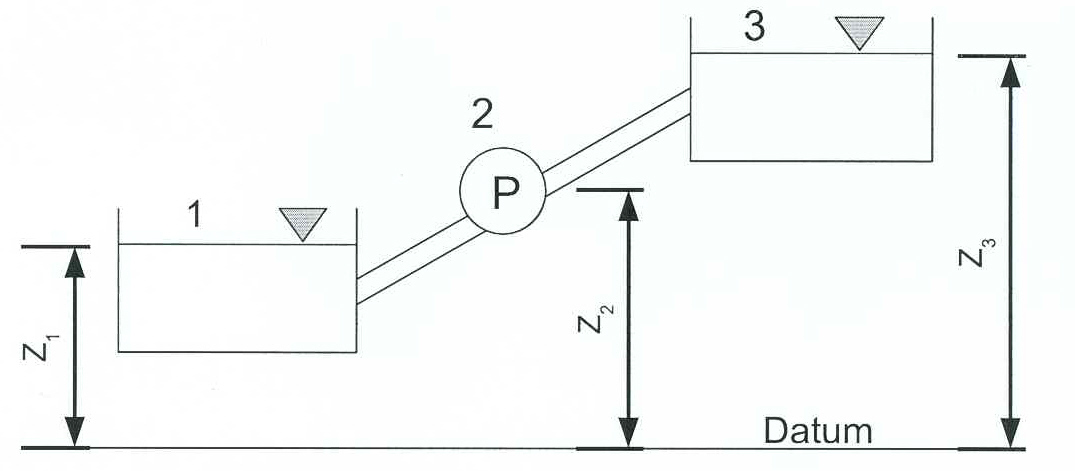
\includegraphics{pumpsystem.jpg}} \caption{Irrigation
water storage system(Finney 2006)}
\end{center}
\end{figure}

The goal of this exercise is to determine the minimum pipe diameter
needed in this situation given pump input power ($h_p$) and pump
efficiency ($e$).
\section {Methodology}
The flow of water between the two reservoirs is determined by this
general energy equation
\begin{singlespace}
\begin{equation}
\frac{p_1}{\gamma}+\frac{v_1^2}{2g}+Z_1-h_f+E_p=\frac{p_3}{\gamma}+\frac{v_3^2}{2g}+Z_3
\end{equation}
where

\begin{center}
\begin{tabular}{rcl}
$p_i$&=& pressure at point $i$\\
$\gamma$&=& specific weight of the fluid\\
$v_i$&=& fluid velocity at point $i$\\
$h_f$&=&friction losses\\
$E_p$&=& energy head supplied by pump (P)
\end{tabular}
\end{center}
\end{singlespace}

By various assumptions, this equation can be shown to simplify to
\begin{singlespace}
\begin{equation}
h_f=E_p-h
\end{equation}
where
\begin{center}
\begin{tabular}{rcl}
$h$&=&$Z_3-Z_1$
\end{tabular}
\end{center}
$E_p$ can be determined from
\begin{equation}
E_p=\frac{76.04e\cdot h_p}{\gamma Q}
\end{equation}
where
\begin{center}
\begin{tabular}{rcl}
$Q$&=&flow rate (m$^3$/s)\\
$h_p$&=&pump input power (horsepower)\\
$\gamma$ &=&specific weight of water(kg/m$^3$)\\
$e$&=&pump efficiency\\
$E_p$&=&pump output head(m)
\end{tabular}
\end{center}
\end{singlespace}

All values in (3) are known or given so $E_p$ can be calculated and
then substituting into (2), $h_f$ can be determined.

$h_f$ can be related to other known values including the pipe
diameter (d) in the Darcy-Weisbach equation for head loss due to
friction by
\begin{singlespace}
\begin{equation}
h_f=f\frac{lv^2}{2dg}
\end{equation}
where
\begin{center}
\begin{tabular}{rcl}
$h_f$&=&friction head loss(m)\\
$f$&=&Darcy-Weisbach friction coefficient (m$^3$/s)\\
$l$ &=&pipe length (m)\\
$v$&=&fluid velocity (m/s)\\
$d$&=&pipe diameter (m)\\
$g$&=&acceleration due to gravity(9.81 m/s$^2$)(Finney 2006)
\end{tabular}
\end{center}
\end{singlespace}

The Colebrook and White equation further relates  the friction
coefficient $f$ to pipe diameter $d$
\begin{equation}
\frac{1}{\sqrt{f}}=-2\log_{10}\left(\frac{k}{3.7d}+\frac{2.51}{Re\sqrt{f}}\right)
\end{equation}
where
\begin{center}
\begin{tabular}{rcl}
$k$&=& absolute roughness of the pipe (m)\\
$Re$&=& Reynolds number ($vd$/$\nu$)\\
$\nu$&=& fluid viscosity (m$^2$/s)(Finney 2006) \\
\end{tabular}
\end{center}

The roots of (5) can be determined by rearranging (5) so that it
equals $0$. Solving (4) for $f$ and substituting into (5) will yield
an equation in the unknown, $d$
\begin{equation}
\frac{Q}{\pi\sqrt{\frac{h_fgd^5}{8l}}}+2\log_{10}\left(\frac{k}{3.7d}+\frac{.6275\nu}{\sqrt\frac{2h_fgd^3}{8l}}\right)=0
\end{equation}
the value of $d$ that satisfies this equation will be the minimum
pipe diameter to use in this situation.

(6) has no analytical solution so in order to determine the roots of
(6), numerical methods must be employed.  Finding the derivative of
(6) is not a simple calculation, so Newton's method is an
undesirable root finding method.  The bisection method is too slow
and it may be difficult to bracket the root.  The secant method is
the best method for numerical root finding in this situation.  This
method requires only one functional evaluation per iteration,
requires no derivative to be taken, and requires the least
computational effort of the three methods. The secant method
algorithm takes the form
\begin{equation}
x_{k+1}=x_k-f(x_k)\left[\frac{x_{k}-x_{k-1}}{f(x_k)-f(x_{k-1})}\right]
\end{equation}
where
\begin{center}
\begin{tabular}{rcl}
$x_{k+1}$&=& updated root estimate\\
$x_k$&=& first root estimate\\
$x_{x-1}$&=& second root estimate
\end{tabular}
\end{center}

In program pipe dim (appendix A) the secant method is utilized to
find the root of (6).

\begin{figure}[!h]
\caption{sample secant method algorithm taken from program pipe dim}
\begin{Verbatim}[frame=single]
do
    xnew=xold-(fxold*((xold-xolder)/(fxold-fxolder)))
              !root update
    fxnew=f(xnew)
    if(stopping criteria met)
      exit
    end if
    fxolder=fxold    !swap values to reduce number
    fxold=fxnew      !of functional evaluations
    xolder=xold
    xold=xnew
end do
\end{Verbatim}
\end{figure}
The values of the variables are swapped after every iteration to
reduce the number of functional evaluations.  Stopping criteria
includes a max iteration test, slow progress test, divergence test,
and root found test.

\section{Application}
The pipe diameter (d) is dependent on the value of various
parameters (Table 1) which are know in this problem.

\begin{table}[!h]
\caption{Parameters associated with determining pipe diameter}
\begin{center}
\begin{tabular}{|l|l|l|}\hline
\multicolumn{1}{|c|}{\bf Parameter} & \multicolumn{1}{c|}{\bf
Variable} & \multicolumn{1}{c|}{\bf Value} \\ \hline Change in
height
& $h$ & 10m \\ \hline Energy head supplied by pump & $E_p$ & 15.24m \\
\hline Flow rate & $Q$ & .3m$^3$/s \\ \hline Specific weight of
water &
$\gamma$ & 998.2kg/m$^3$ \\ \hline Friction head loss & $h_f$ & 5.24m \\
\hline Pipe length & $l$ & 95m \\ \hline Absolute roughens & $k$ &
2.591x10-4m \\ \hline Fluid viscosity & $\nu$ & 1.007x10$^-6$m$^2$/s \\
\hline Acceleration due to gravity & $g$ & 9.81m/s$^2$) \\ \hline
Epsilon 1 & $\varepsilon_1$ & 10$^-6$ \\ \hline Epsilon 2 & $\varepsilon_2$ & 10$^-9$ \\
\hline
\end{tabular}
\end{center}
\end{table}

\newpage To test the sensitivity of the model, different parameters can be
varied (Table 2).

\begin{table}[!h]
\begin{center}
\caption{Variation of Parameters} \vspace{.2in}
\begin{tabular}{|c|l|l|l|l|}\hline
\bf Run \# & \multicolumn{1}{c|}{\bf Variable} &
\multicolumn{1}{c|}{\bf Initial value} & \multicolumn{1}{c|}{\bf New
value} & \multicolumn{1}{c|}{\bf Percent varied} \\ \hline
1 & e & 60\% & 66\% & 10\% \\
2 &  &  & 54\% & -10\% \\ \hline
3 & $h_p$ & 100 $hp$ & 110 & 10\% \\
4 &  &  & 90 & -10\% \\ \hline
5 & Q & .3 m$^3$ & 0.33 & 10\% \\
6 &  &  & 0.27 & -10\% \\ \hline
7 & $h_f$ & 5.24 m & 5.764 & 10\% \\
8 &  &  & 4.716 & -10\% \\ \hline
9 & $l$ & 95 m & 104.5 & 10\% \\
10 &  &  & 85.5 & -10\% \\ \hline
11 & $k$ & 0.0002591 & 0.00028501 & 10\% \\
12 &  &  & 0.00023319 & -10\% \\ \hline
13 & $\varepsilon_1$ & $10^{-6}$ & $11^{-6}$ & 10\% \\
14 &  &  & $9^{-7}$ & -10\% \\ \hline
15 & $\varepsilon_2$ & $10^{-8}$ & $11^{-8}$ & 10\% \\
16 &  &  & $9^{-9}$ & -10\% \\ \hline
\end{tabular}
\end{center}
\end{table}

\newpage
\section{Results}
Plugging the values form table 2 into (6) and graphing $y$ as a
function of pipe diameter ($d$) yields a graph with one apparent
root (Figure 3).  Utilizing the secant method within program pipe
dim reveals the root is approximately .3038 m.  This value is the
minimum pipe diameter that should be used between the two
reservoirs.
\begin{figure}[!h]
\begin{center}
\scalebox{.65}{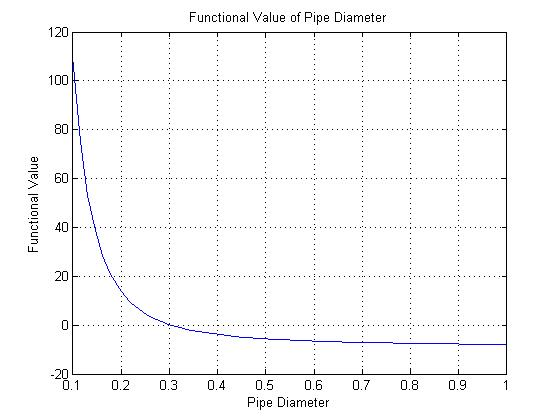
\includegraphics{pipe_function_plot.jpg}}
\caption{Plot of pipe diameter function}
\end{center}
\end{figure}

The sensitivity analysis reveals how $d$ changes with the variation
of parameters (Table 3).

\begin{table}[!h]
\caption{Results of variation of parameters (all values tested with
initial root estimates of .25,.26)}
\begin{center}
\begin{tabular}{|c|l|l|l|l|l|}\hline
\multicolumn{1}{|l|}{\bf Run \#} & \multicolumn{1}{l}{\bf Variable}
& \bf New value & \bf Percent varied & \bf Pipe diameter &
\multicolumn{1}{c|}{\bf Variation} \\ \hline
1 & e & 66\% & 10\% & 0.2893 & 4.71\% \\
2 &  & 54\% & -10\% & 0.3245 & 6.88\% \\ \hline
3 & $h_p$ & 110 & 10\% & 0.2893 & 4.71\% \\
4 &  & 90 & -10\% & 0.3245 & 6.88\% \\ \hline
5 & Q & 0.33 & 10\% & 0.3342 & 10.08\% \\
6 &  & 0.27 & -10\% & 0.2766 & 8.89\% \\ \hline
7 & $h_f$ & 5.764 & 10\% & 0.3093 & 1.89\% \\
8 &  & 4.716 & -10\% & 0.3214 & 5.86\% \\ \hline
9 & $l$ & 104.5 & 10\% & 0.3091 & 1.81\% \\
10 &  & 85.5 & -10\% & 0.2974 & 2.04\% \\ \hline
11 & $k$ & 0.00028501 & 10\% & 0.3048 & 0.40\% \\
12 &  & 0.00023319 & -10\% & 0.3021 & 0.49\% \\ \hline
13 & $\varepsilon_1$ & $11^{-6}$ & 10\% & 0.3038 & 0\% \\
14 &  & $9^{-7}$ & -10\% & 0.3038 & 0\% \\ \hline
15 & $\varepsilon_2$ & $11^{-8}$ & 10\% & 0.3038 & 0\% \\
16 &  & $9^{-9}$ & -10\% & 0.3038 & 0\% \\ \hline
\end{tabular}
\end{center}
\end{table}

Varying the efficiency ($e$) and the horsepower ($h_p$) affects the
the pipe diameter ($d$) in the same way because they are of equal
proportion in (3). $10.08\%$, The largest variation of the result
was seen when varying the flow rate $Q$ by positive $10\%$.  A
$10\%$ increase in the flow rate necessitates a 3 cm increase in the
pipe diameter. A $10\%$ variation if the absolute roughness ($k$)
has the least effect on the outcome.  A variation of both epsilon
values ($\varepsilon_1$,$\varepsilon_2$) by $\pm10\%$ had no effect
on the resultant pipe diameter.
\newpage
\section{Conclusions}
\begin{itemize}
  \item{The minimum pipe diameter that can be used with a $60\%$ efficient, 100hp pump is .3038 m}
  \item{The absolute roughness ($k$) is the least influential parameter}
  \item{The flow rate ($Q$) is the most influential parameter}
  \item{A $\pm10\%$ variation in the stopping criteria,
  $\varepsilon_1$,$\varepsilon_2$, has no effect on the solution}
\end{itemize}

\section{References}

Finney,Brad. Lab 7 handout, Humboldt State University, Spring 2006.

\appendix
\newcommand{\appsection}[1]{\let\oldthesection\thesection
  \renewcommand{\thesection}{Appendix \oldthesection}
  \section{#1}\let\thesection\oldthesection}
\appsection{\\~Source Code and Program Output} \label{sec:source}

\begin{singlespace}
\begin{Verbatim}[frame=single]
module constants
  double precision,parameter::pi=3.1415926,Q=.3,L=95,h=10,specw=998.2,&
                              visc=.000001007,g=9.81,k=.0002591
  double precision::hf
end module constants

Program pipe_dim
  use constants
  implicit none
  double precision::di,x1,x2,hp,e
  integer::tries
  logical::success
  interface
    subroutine secant(xold,xolder,maxit,epsi1,epsi2,root,numit,exitflag,f)
      double precision,intent(inout)::xold,xolder
      double precision,intent(in)::epsi1,epsi2
      double precision,intent(out)::root
      double precision::xnew,fxnew,fxold,fxolder
      integer,intent(in)::maxit
      integer,intent(out)::numit
      logical,intent(out)::exitflag
      interface
        function f(x)
          double precision::x
          double precision::f
        end function f
      end interface
    end subroutine secant
  end interface
  interface
    function f(x)
      double precision::x
      double precision::f
    end function f
  end interface

  !This program will find the optimal pipe diameter between two water
  !storage tanks at different heights with a pump in between as described
  !in engr 325 lab assignment 7.  To find the pipe diameter this program will
  !call a root finding subroutine which will call a function subprogram to
  !evaluate the given pipe diameter function.
  !
  !variable list:
  ! local variables:
  !hf      =friction loss(pump energy-change of potential) (m)
  !specw   =specific weight of water (kg/m^3)
  !Q       =flow rate(m^3/s)
  ! inputs:
  !hp      =horsepower of pump (horsepower)
  !e       =pump efficiency
  !x1,x2   =initial pipe diameter guesses (m)
  ! outputs:
  !di      =pipe diameter (m)
  !tries   =number of iterations the rootfinding subroutine went through to
  !         determine the root
  !success =value is .true. if root successfully found,else .false.

  write(*,*)"This Program will calculate..."
  write(*,*)"Enter the horsepower of the pump"
  read(*,*)hp
  write(*,*)"Enter the efficiency of the pump"
  read(*,*)e
  hf=(76.04d0*e*hp)/(specw*Q)-h
  !write(*,*)"hf=",hf
  write(*,*)"Enter the first root estimate"
  read(*,*)x1
  write(*,*)"Enter the second root estimate"
  read(*,*)x2
  call secant(x1,x2,20,.00001d0,.00000001d0,di,tries,success,f)
  if(success)then
    write(*,"(a18,x,f10.5)")"The pipe diameter=",di
    write(*,"(a7,x,i2,x,a27)")"It took",tries,"iterations to find the root"
  end if
  stop
end program pipe_dim


subroutine
secant(xold,xolder,maxit,epsi1,epsi2,root,numit,exitflag,f)
  implicit none
  double precision,intent(inout)::xold,xolder
  double precision,intent(in)::epsi1,epsi2
  double precision,intent(out)::root
  double precision::xnew,fxnew,fxold,fxolder     !local variables
  integer,intent(in)::maxit
  integer,intent(out)::numit
  logical,intent(out)::exitflag
  interface
    function f(x)
      double precision::x
      double precision::f
    end function f
  end interface

  !This is a general rootfinding subroutine that employs the secant method
  !it must be used in conjunction with an external function subprogram that
  !will evaluate the function in question
  !
  !variable list:
  ! local variables:
  !xnew      =updated root estimate
  !fxnew     =function evaluated at updated root estimate
  !fxold     =function evaluated at old root estimate
  !fxolder   =function evaluated at older root estimate
  ! inputs:
  !xold      =old root estimate
  !xolder    =older root estimate
  !epsi1     =stopping criteria for root found, if f(xnew)<epsi1 then
  !           root found
  !epsi2     =stopping criteria for slow progress, if abs(xold-xolder)<epsi2)
  !           then too slow
  !maxit     =maxumum allowable iterations subroutine will perform
  !           until it exits
  ! outputs:
  !root      =value of particular found root
  !numit     =records number of iterations done by subroutine
  !exitflag  =value is .true. if root successfully found,else .false.

  numit=0
  fxold=f(xold)
  fxolder=f(xolder)
  do
    xnew=xold-(fxold*((xold-xolder)/(fxold-fxolder)))
              !fxold*((xold-xolder)/(fxold-fxolder)) is root update
    fxnew=f(xnew)
    !write(*,*)"fxnew=",fxnew
    numit=numit+1
    if(abs(fxnew)<epsi1)then
      write(*,*)"root found"
      root=xnew
      exitflag=.true.
      return
      exit
    else if(numit>maxit)then
      write(*,*)"No root found (max iterations exceeded), try a better guess."
      exitflag=.false.
      return
      exit
    else if(abs(xold-xolder)<epsi2)then
      write(*,*)"No root found (progress too slow),try better guess."
      exitflag=.false.
      return
    else if ((abs(xnew-xold))>=(abs(xold-xolder)) .and. numit/=1)then
      write(*,"(a38,x,i2,x,a28)")"No root found (solution diverged after",numit,&
                                 "iterations),try better guess."
      exitflag=.false.
      return
    end if
    fxolder=fxold    !swap values to reduce number of functional evaluations
    fxold=fxnew
    xolder=xold
    xold=xnew
    !write(*,*)"fxolder=",fxolder
    !write(*,*)"fxold=",fxold
    !write(*,*)"xolder=",xolder
    !write(*,*)"xold=",xold
  end do
end subroutine secant


function f(d)
  use constants
  double precision,intent(in)::d
  double precision::A,v,fdw,Re,f    !local variables except f

  !This function subprogram evaluates the diameter function below
  !variable list:
  ! local variables
  !A     =cross sectional area of the pipe (m^2)
  !v     =fluid velocity (m/s)
  !fdw   =Darcy-Weisbach friction coefficient (m^2/s)
  !Re    =Reynolds number (dimensionless)
  !pi    =pi (3.1415926)
  !Q     =flow rate(m^3/s)
  !hf    =friction loss(pump energy-change of potential) (m)
  !g     =gravitational constant (9.81 m/s^2)
  !L     =pipe length (m)
  !visc  =fluid viscocity (m^2/s)
  ! inputs:
  !d     =pipe diameter (m)
  ! outputs:
  !f     =function value at given pipe diameter

  A=(pi*d**2d0)/4d0
  v=(4d0*Q)/(pi*d**2d0)
  fdw=(2d0*hf*g*d)/(L*v**2d0)
  Re=(v*d)/(visc)
   !write(*,*)"A=",A
   !write(*,*)"v=",v
   !write(*,*)"fdw=",fdw
   !write(*,*)"re=",Re
  f=-1d0/sqrt(fdw)-2d0*log10(k/(3.7d0*d)+2.51d0/(Re*sqrt(fdw)))
   !f=-d**(2d0)+1  !check function root=1
end function f

\end{Verbatim}
\end{singlespace}

\noindent This was typeset with \LaTeX
\end{document}
